\section{Разработка компактной мобильной антенны.} 

На сегодняшний день известно множество конструкций антенн, соответствующих заданным требованиям. Одними из самых распространённых и при этом простых в изготовлении являются спиральные антенны нормального излучения. Расчёт размеров антенны будем проводить с помощью LibreOffice Calc. Оригинал таблицы будет находиться в репозитории проекта, здесь же приведем лишь результаты расчёта.

\subsection{Расчёт размеров антенны.}

Антенна будет разрабатываться для частоты $f_c=\frac{864+870}{2}=867$~МГц (длина волны $\lambda\approx345$~мм)


\begin{longtblr}[
	caption = {Задаваемые параметры антенны},
	label = {table:antenna-set-params}
	]{
		colspec={Q[5,l,m]Q[3,l,m]Q[3,l,m]},
		width=0.8\textwidth,
		vlines,hlines,
		vspan=even,
		rowhead=1,
		row{1-2}={font=\bfseries}
	}
	%%%%%%%%%%%%%%%%%%%%%%%%%%%%%%%%%%%%%%%%%%%%%%%
	\SetCell[r=2]{c} Параметр & \SetCell[c=2]{c} Значение \\	
	& \SetCell[c=1]{c} Вариант 1 & \SetCell[c=1]{c}Вариант 2 \\
	%%%%%%%%%%%%%%%%%%%%%%%%%%%%%%%%%%%%%%%%%%%%%%%%
	Длина запитки $l_{feed}$ & \SetCell[c=2]{l} 3~мм \\
	Длина спирали $l_{helix}$ & \SetCell[c=2]{l} $\lambda/4-l_{feed}=83,35$~мм \\
	Диаметр проводника & \SetCell[c=2]{l} 1~мм \\
	Диаметр спирали & 5~мм & 3~мм \\
	Шаг намотки (расстояние между центрами витков) & \SetCell[c=2]{l} 1,2~мм \\
\end{longtblr}


\begin{longtblr}[
	caption = {Рассчитанные параметры антенны},
	label = {table:antenna-counted-params}
	]{
		colspec={Q[5,l,m]Q[3,l,m]Q[3,l,m]},
		width=0.8\textwidth,
		vlines,hlines,
		vspan=even,
		rowhead=1,
		row{1-2}={font=\bfseries}
	}
	%%%%%%%%%%%%%%%%%%%%%%%%%%%%%%%%%%%%%%%%%%%%%%%
	\SetCell[r=2]{c} Параметр 		& \SetCell[c=2]{c} Значение \\	
	& \SetCell[c=1]{c} Вариант 1 	& \SetCell[c=1]{c} Вариант 2 \\
	%%%%%%%%%%%%%%%%%%%%%%%%%%%%%%%%%%%%%%%%%%%%%%%%
	Высота спирали 			& \SetCell[c=1]{c} 6,35 мм 	& \SetCell[c=1]{c} 10,53 мм \\
	Число витков 			& \SetCell[c=1]{c} 5,291 	& \SetCell[c=1]{c} 8,773 \\
	Угол намотки спирали	& \SetCell[c=1]{c} $4,37^o$ & \SetCell[c=1]{c} $7,26^o$ \\
\end{longtblr}

\subsection{Моделирование антенны в CST Studio Suite.}

Для создания модели спирали использовался встроенный скрипт, для запитки — цилиндр. Все острые углы и неестественные неравномерности были сглажены. 

Для учета влияния платы была создана модель, повторяющая её контуры.

Итоговые симуляционные модели показаны на Рисунке \ref{fig:cst-model-board}.

\begin{figure}[H]
	\centering
	\begin{subfigure}[c]{0.49\textwidth}
		\centering
		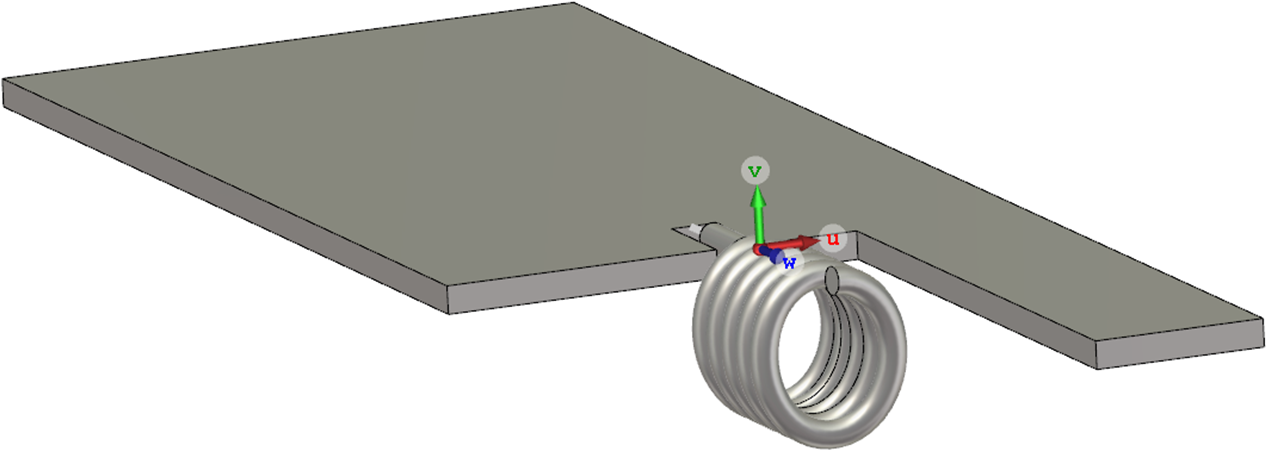
\includegraphics[width=\textwidth,height=12em,keepaspectratio]{cst-model-board1.png}
		\caption{}%
		\label{}
	\end{subfigure}
	\hfill
	\begin{subfigure}[c]{0.49\textwidth}
		\centering
		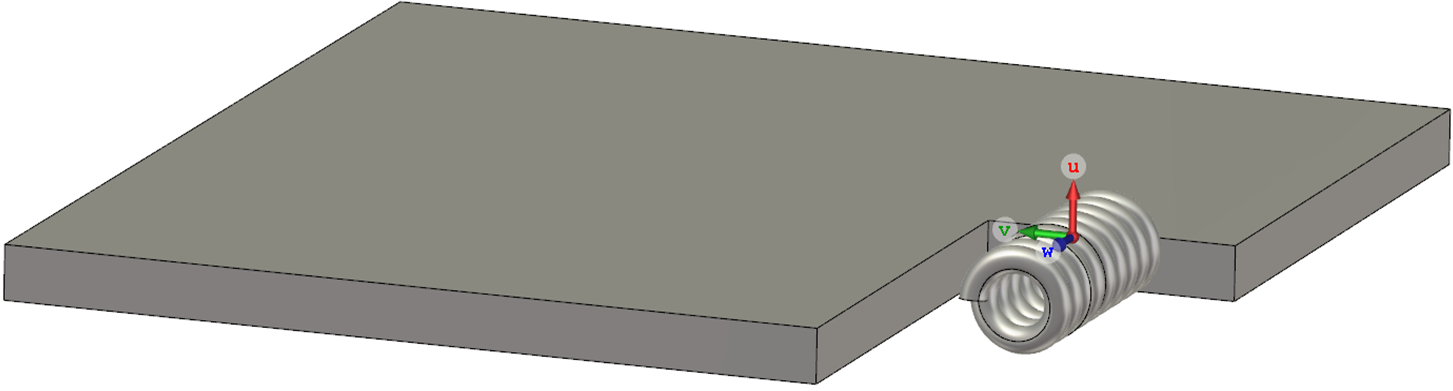
\includegraphics[width=\textwidth,height=12em,keepaspectratio]{cst-model-board2.png}
		\caption{}%
		\label{}
	\end{subfigure}
	\caption{Итоговые модели для симуляции.}
	\label{fig:cst-model-board}
\end{figure}

На Рисунке \ref{fig:cst-farfield-3d} можно увидеть результаты моделирования в объемном отображении. Как видно, $K_y$ антенны равен 1.81 дБи, и излучение является тороидальным, что соответствует теории. Положение нуля зависит от длины антенны и размеров “земли”.

\begin{figure}[H]
	\centering
	\begin{subfigure}[t]{0.49\textwidth}
		\centering
		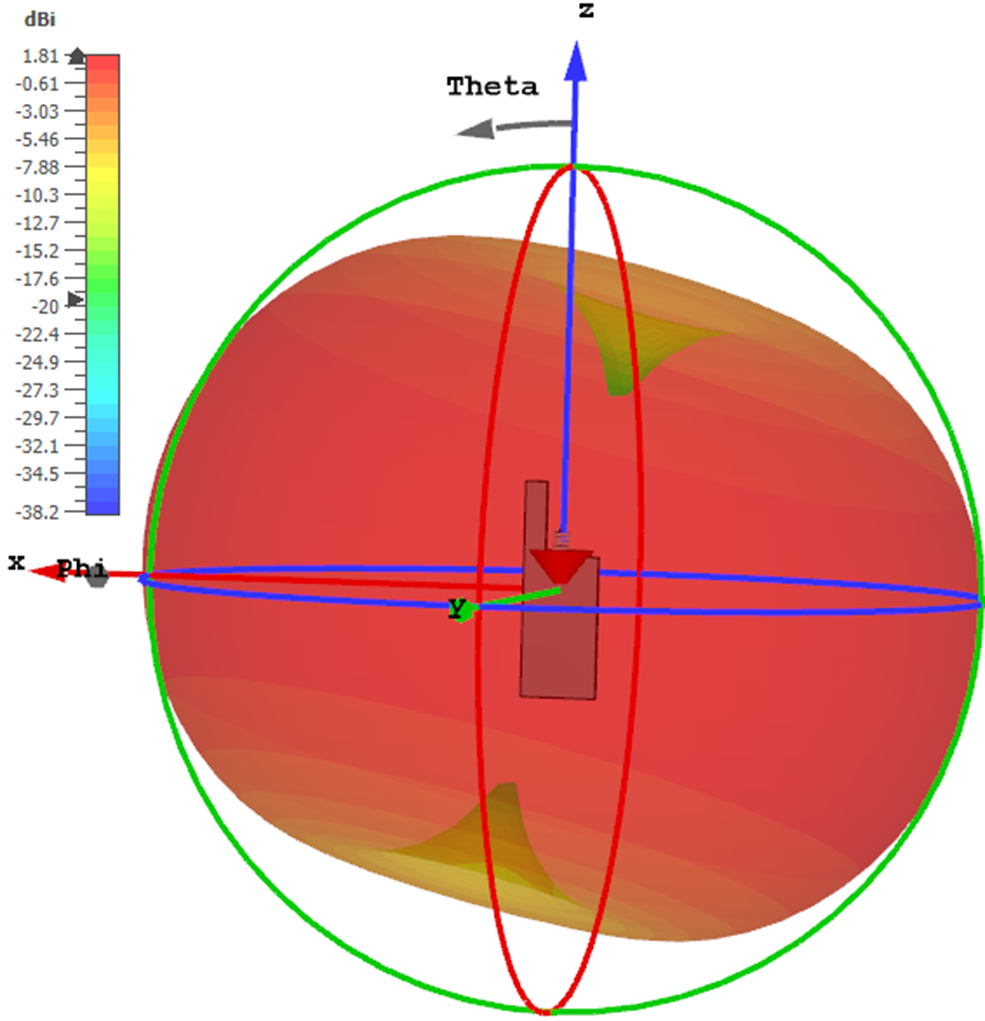
\includegraphics[width=\textwidth,height=17em,keepaspectratio]{cst-farfield-3d1.png}
		\caption{}%
		\label{}
	\end{subfigure}
	\hfill
	\begin{subfigure}[t]{0.49\textwidth}
		\centering
		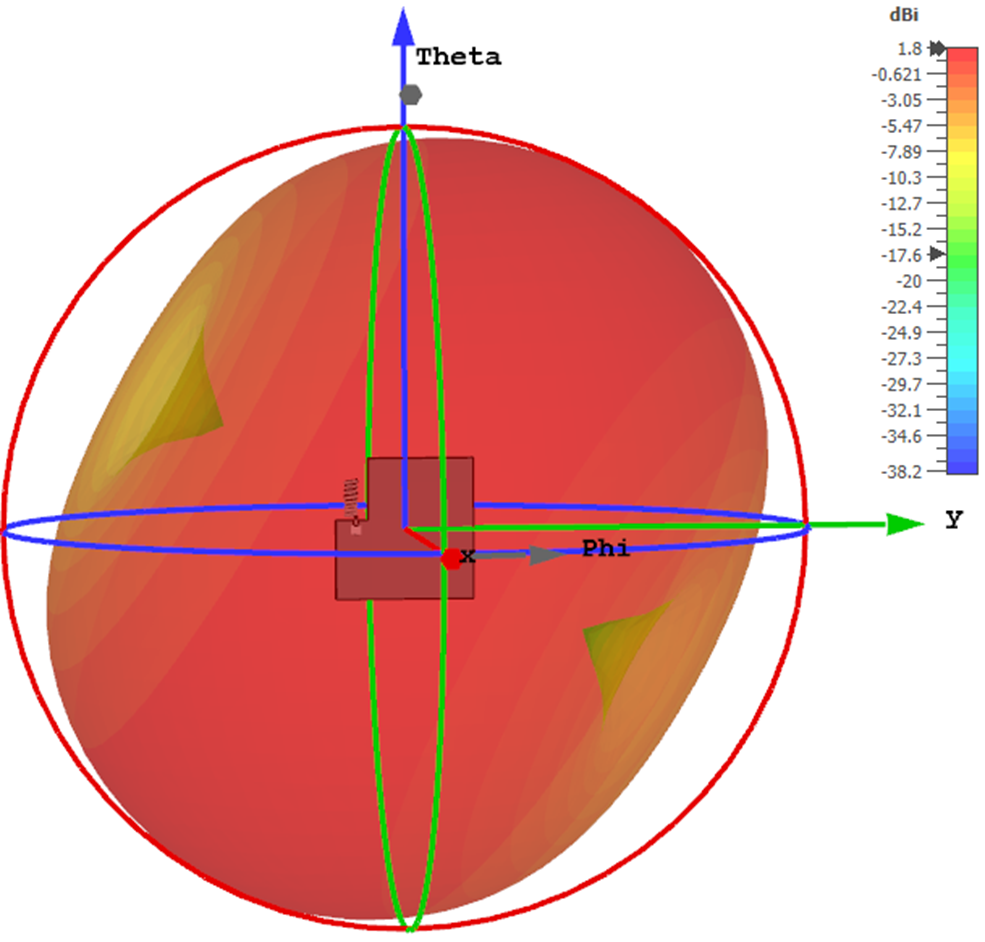
\includegraphics[width=\textwidth,height=17em,keepaspectratio]{cst-farfield-3d2.png}
		\caption{}%
		\label{}
	\end{subfigure}
	\caption{Результаты моделирования поля в дальней зоне. ДН.}
	\label{fig:cst-farfield-3d}
\end{figure}

Дополнительно приведём срез диаграммы направленности (ДН) в плоскости oXZ.

\begin{figure}[H]
	\centering
	\begin{subfigure}[t]{0.49\textwidth}
		\centering
		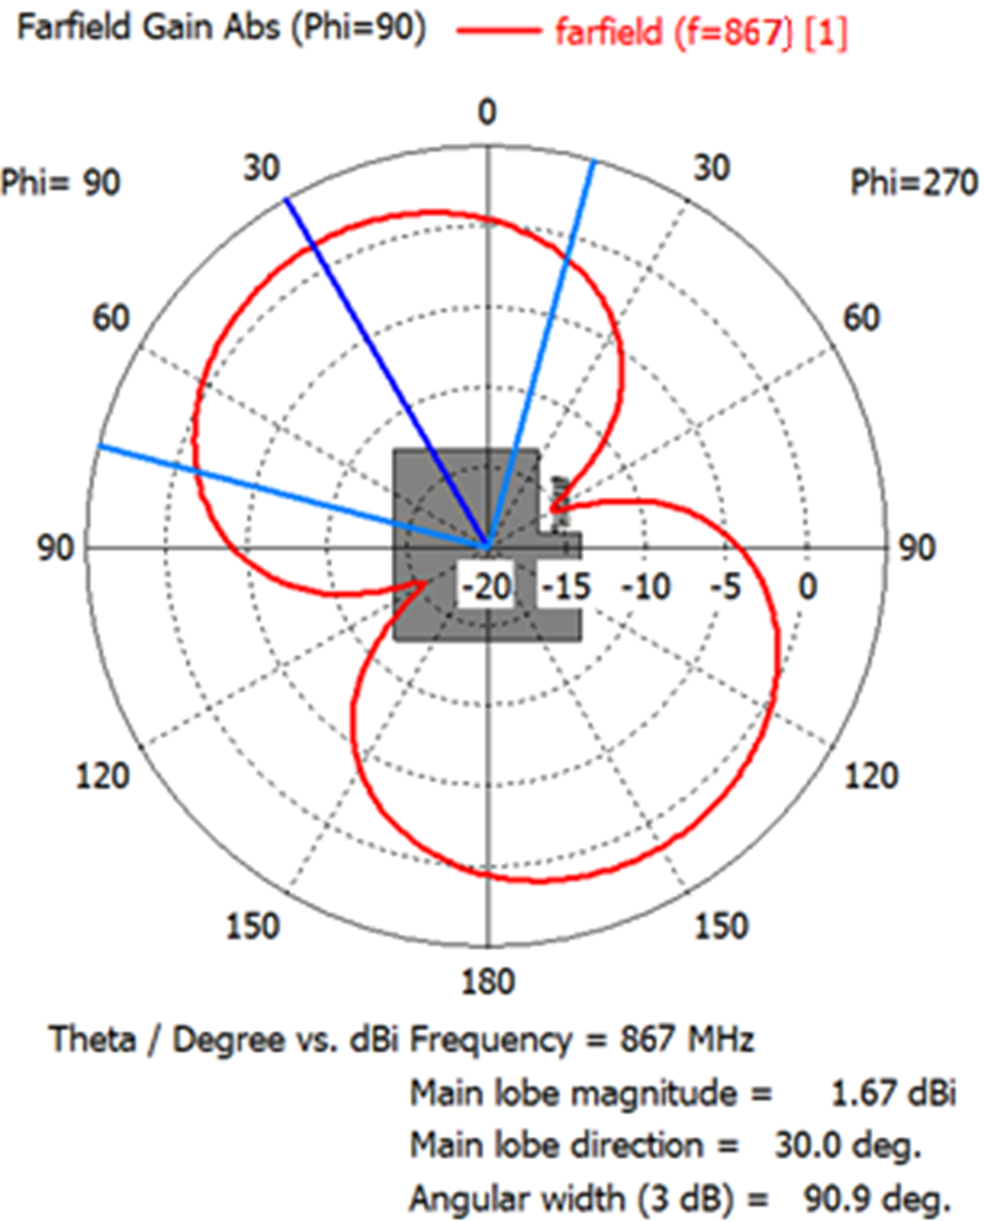
\includegraphics[width=\textwidth,height=17em,keepaspectratio]{cst-farfield-2d1.png}
		\caption{}%
		\label{}
	\end{subfigure}
	\hfill
	\begin{subfigure}[t]{0.49\textwidth}
		\centering
		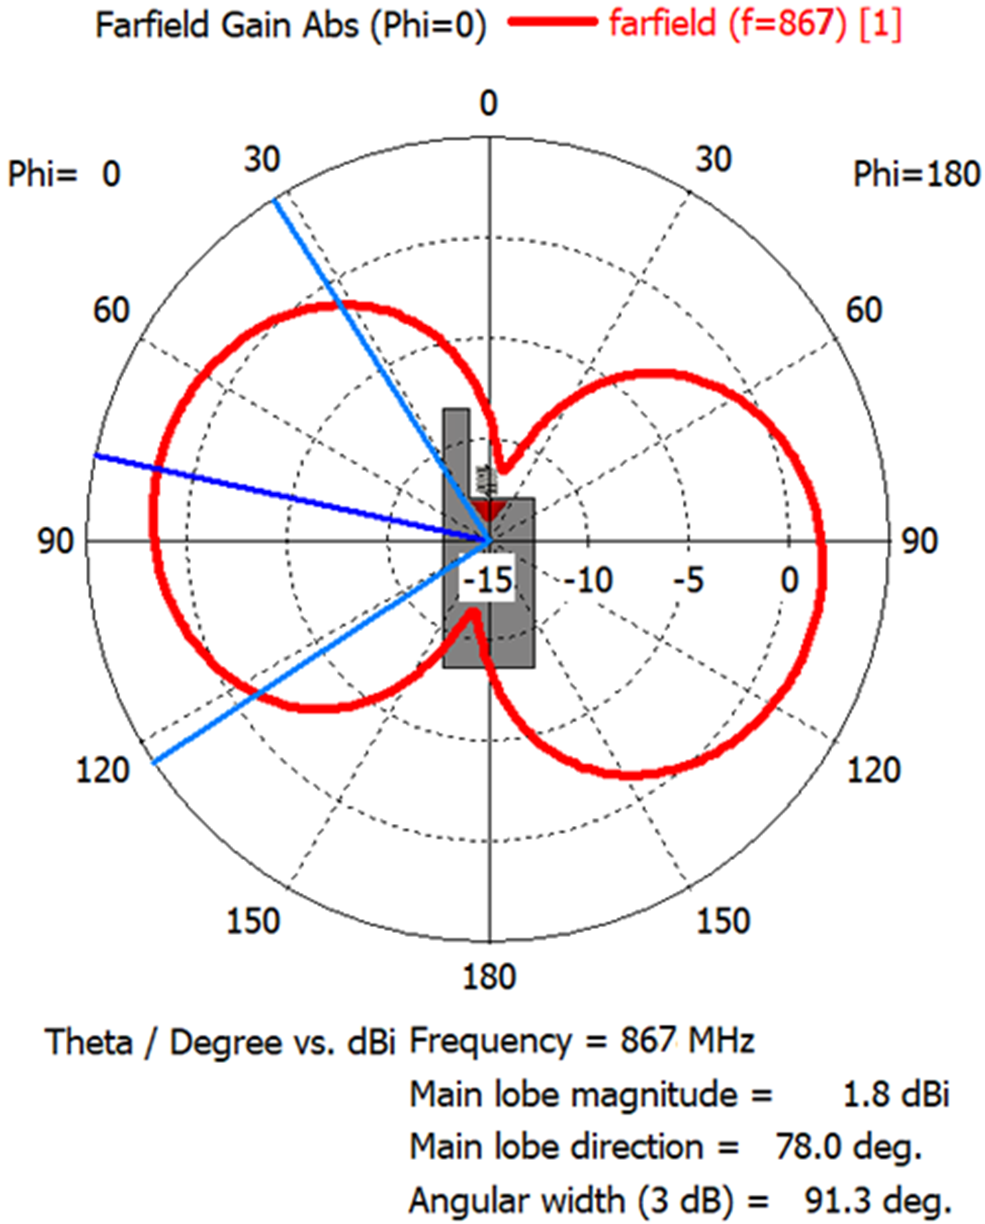
\includegraphics[width=\textwidth,height=17em,keepaspectratio]{cst-farfield-2d2.png}
		\caption{}%
		\label{}
	\end{subfigure}
	\caption{Результаты моделирования поля в дальней зоне в плоскости oXZ.}
	\label{fig:cst-farfield-2d}
\end{figure}

Исследуем поляризационную характеристику антенны. Рассмотрим графики $K_y$ антенны для вертикальной (farfield gain theta) и горизонтальной \linebreak(farfield gain phi) поляризации. 

\begin{figure}[H]
	\centering
	\begin{subfigure}[t]{0.49\textwidth}
		\centering
		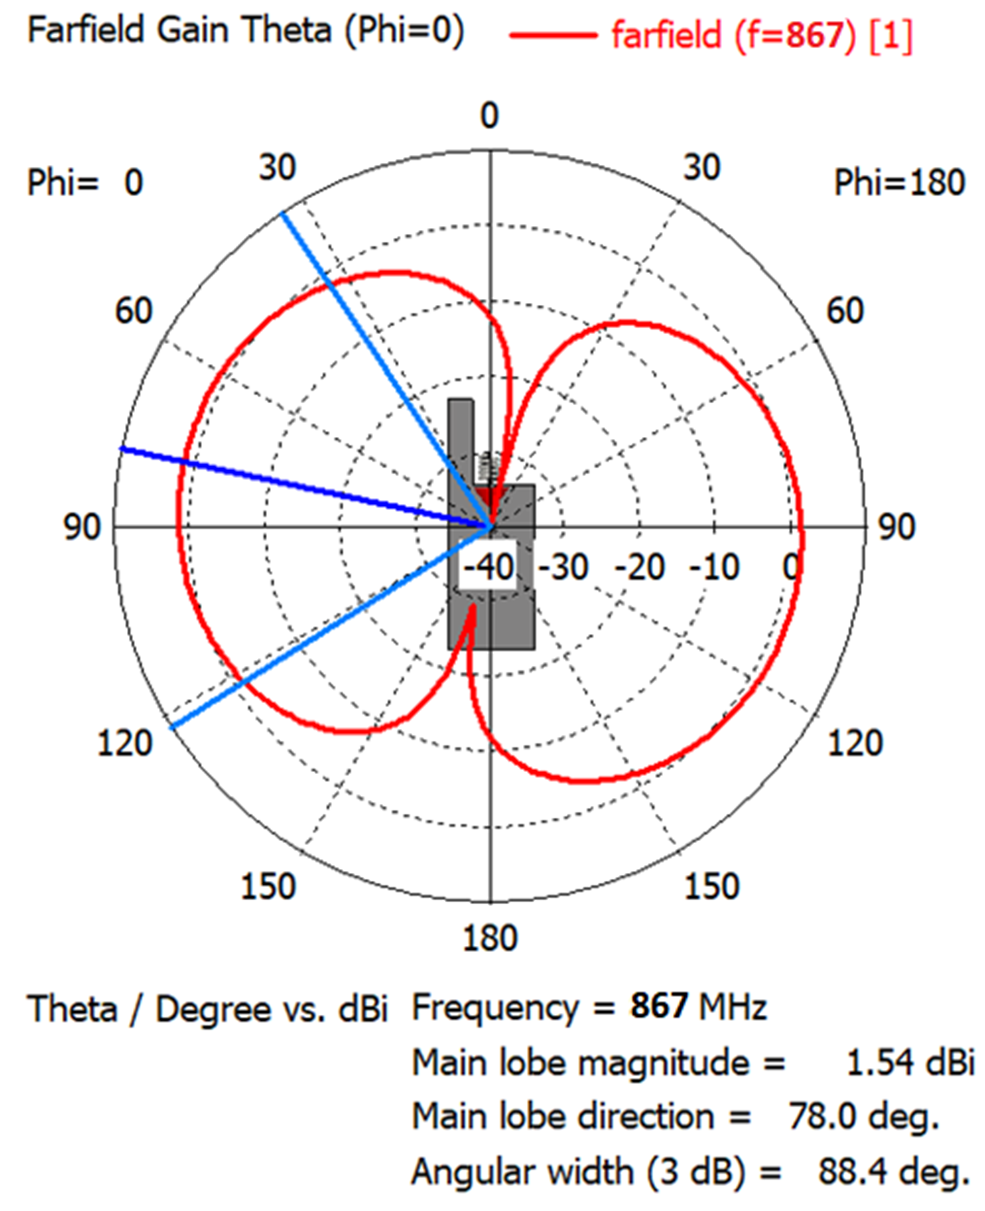
\includegraphics[width=\textwidth,height=17em,keepaspectratio]{CST-antenna1-polarization1.png}
		\caption{}%
		\label{}
	\end{subfigure}
	\hfill
	\begin{subfigure}[t]{0.49\textwidth}
		\centering
		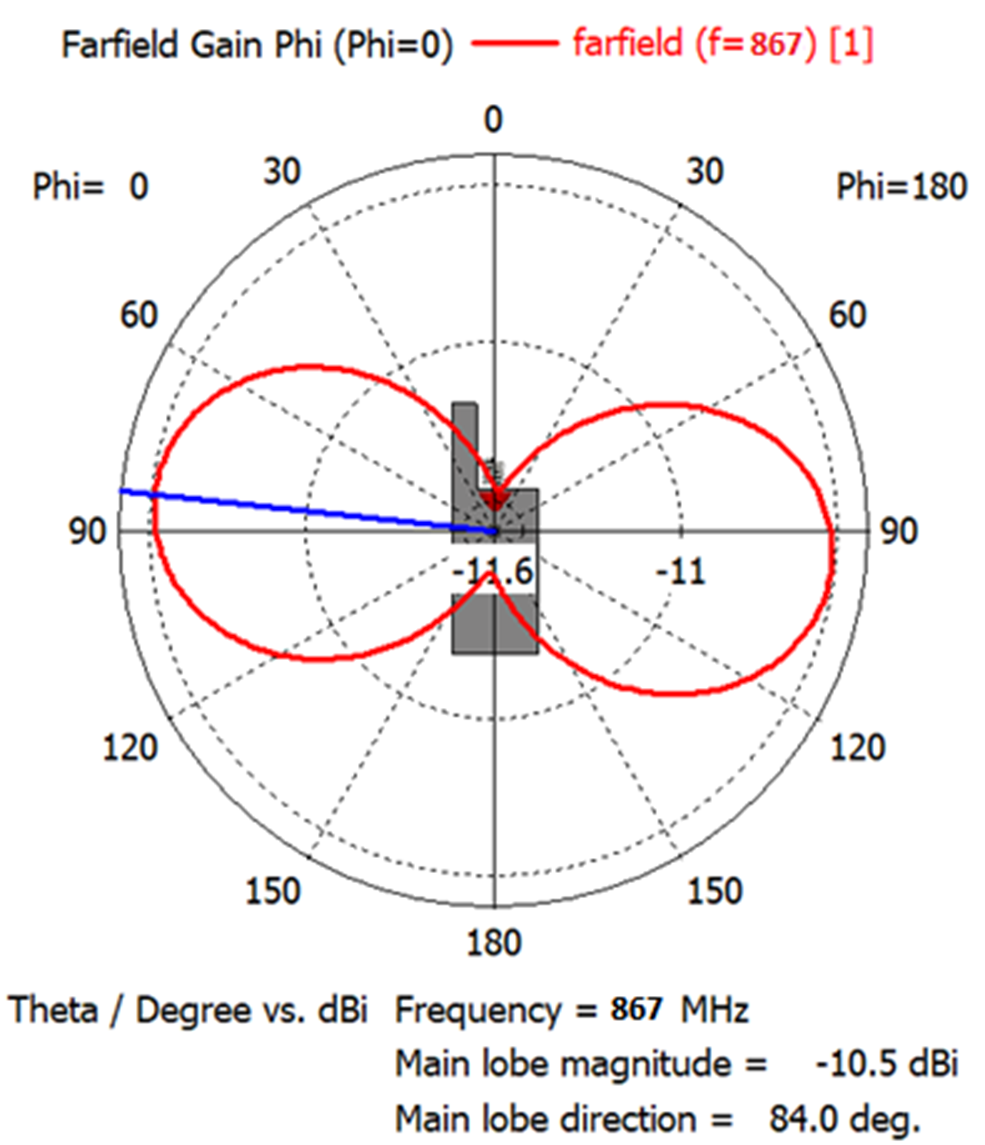
\includegraphics[width=\textwidth,height=17em,keepaspectratio]{CST-antenna1-polarization2.png}
		\caption{}%
		\label{}
	\end{subfigure}
	\caption{Поляризационная характеристика антенны. Вариант 1.}
	\label{fig:CST-antenna1-polarization}
\end{figure}

\begin{figure}[H]
	\centering
	\begin{subfigure}[t]{0.49\textwidth}
		\centering
		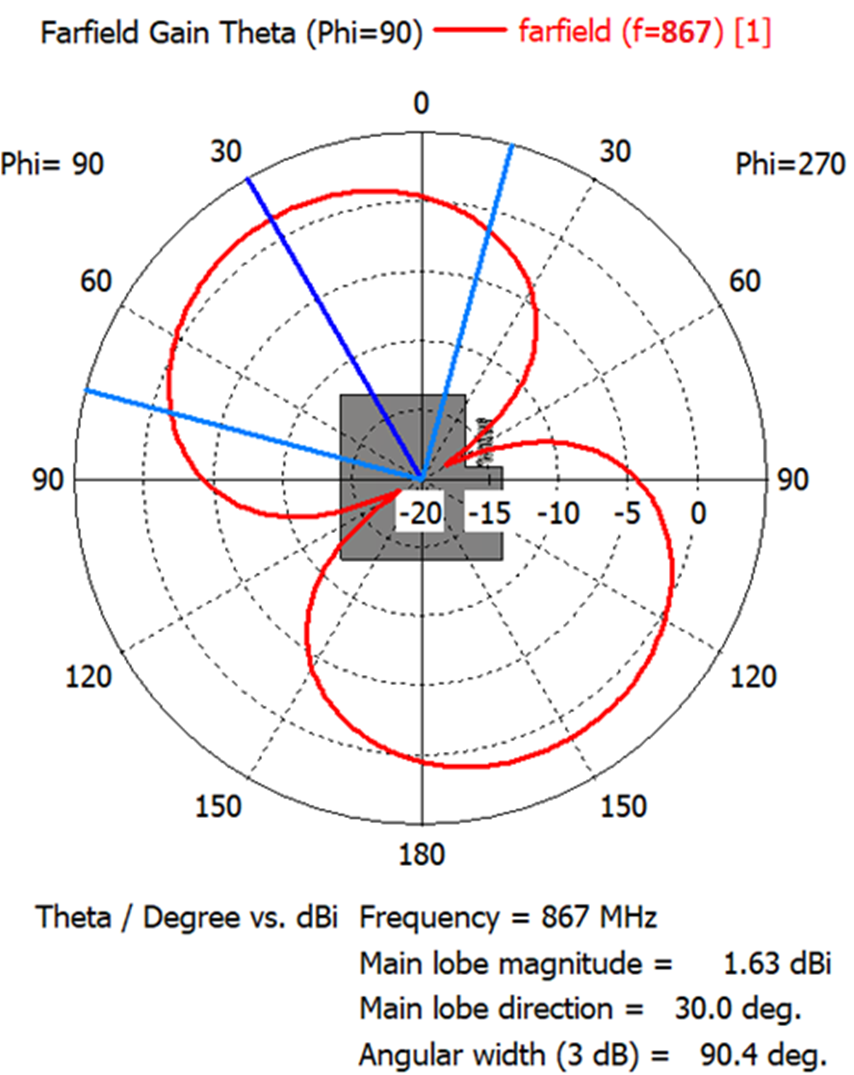
\includegraphics[width=\textwidth,height=17em,keepaspectratio]{CST-antenna2-polarization1.png}
		\caption{}%
		\label{}
	\end{subfigure}
	\hfill
	\begin{subfigure}[t]{0.49\textwidth}
		\centering
		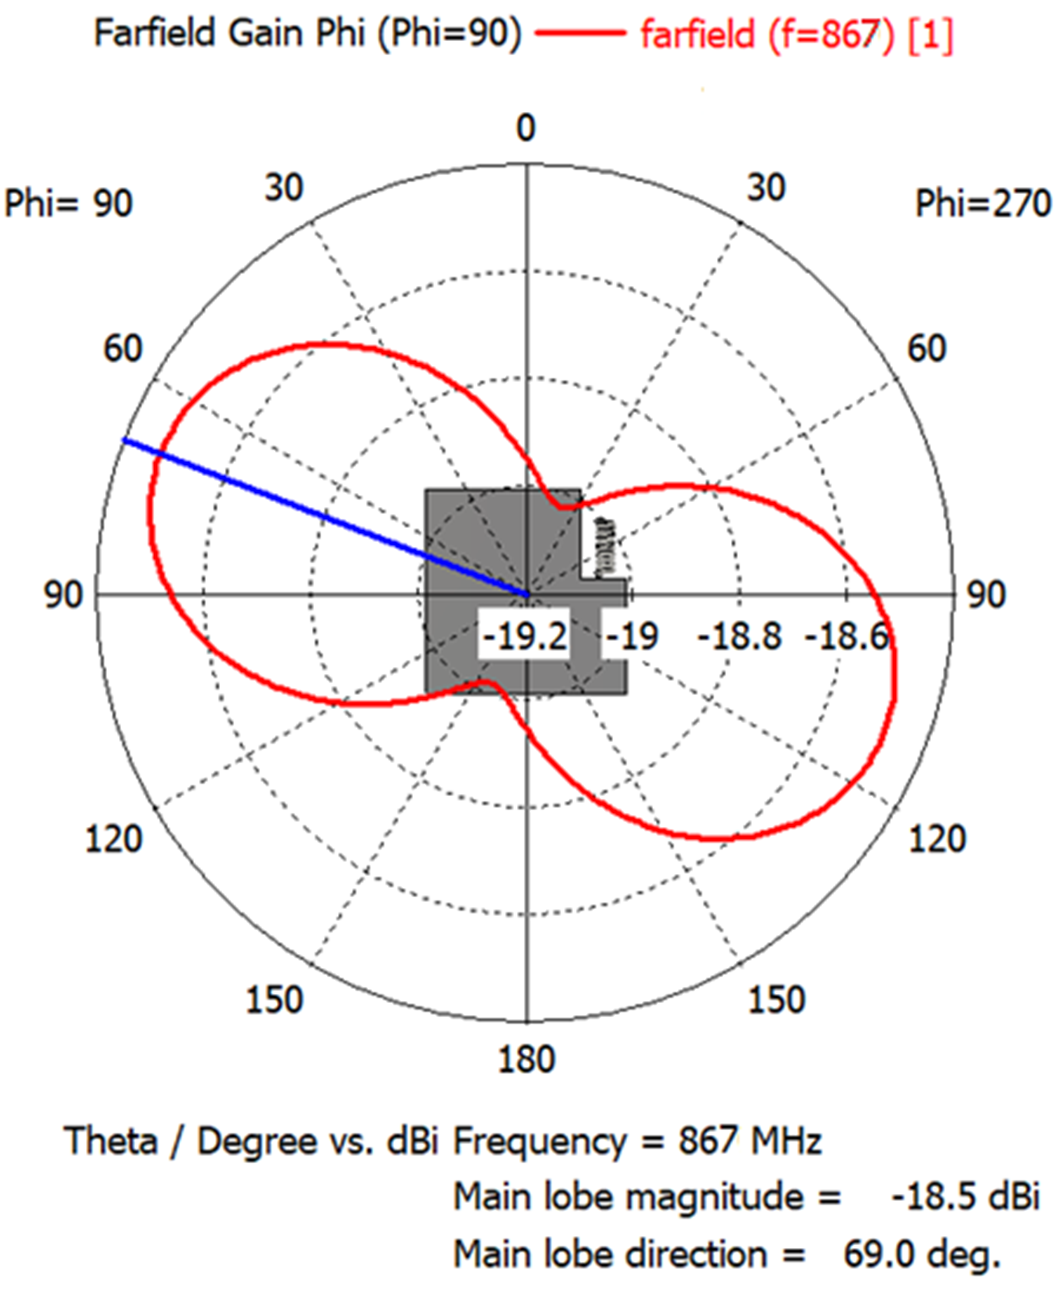
\includegraphics[width=\textwidth,height=17em,keepaspectratio]{CST-antenna2-polarization2.png}
		\caption{}%
		\label{}
	\end{subfigure}
	\caption{Поляризационная характеристика антенны. Вариант 2.}
	\label{fig:CST-antenna2-polarization}
\end{figure}

Исходя из этих данных, антенна является линейно поляризованной по оси Z, и располагать её надо параллельно к антенне базовой станции (в большинстве случаев антенной базовой станции является дипольная либо монопольная антенна с аналогичной поляризационной характеристикой).
